\documentclass[twocolumn,anonymous]{aastex701}
\usepackage{amsmath}
\usepackage{amssymb}
\usepackage{booktabs}
\newcommand{\Btilde}{\widetilde{B}}
\newcommand{\utilde}{\widetilde{u}}
\shorttitle{Magnetized binary Bondi pilot}
\shortauthors{Internal project record}
\begin{document}
\title{A Magnetized Binary Bondi Reservoir with Cyclic Zoom:\\Configuration, Physical Clocks, and an Early Inflow-Equilibrium Audit}
\author{Internal project record}
\begin{abstract}
This working note records the actual configuration and early results of a low-resolution AthenaK magnetized reservoir around an equal-mass, nonspinning circular black-hole binary. The nominal total mass is unity, separation is $32M$, thermal Bondi radius is $500M$, and asymptotic plasma beta is unity. Gas starts as a uniform reservoir at rest in inertial coordinates, not a steady transonic Bondi solution. We distinguish physical puncture excision, artificial cyclic masks, and the external reservoir. The current chain uses hard puncture resets; the available smooth-excision implementation was not enabled. A live check on 2026 October 17 found job 8939546 running in debug-scaling; the retained log reached $t=10208M$ in stage 3. Seven completed jobs provide validated data through $9903.62M$. Only one physical zoom roundtrip has completed, and finest-stage exposure is about $500M$, or $0.44$ binary orbits. Comparing matched phases of startup and first-return visits, near-hole accretion rates increase by factors $4.4$--$4.5$ and shell masses by factors $1.4$--$4.4$. Inflow equilibrium is not established. We provide equations, figures, provenance, and diagnostic limitations so subsequent updates can be assessed consistently.
\end{abstract}
\keywords{Accretion --- Black hole physics --- Magnetohydrodynamics --- Numerical methods}

\section{Status and scope}\label{sec:status}
This is a dated project record, not a converged astrophysical result or a manuscript submitted to ApJ. It concerns the \emph{new magnetic chain}; convergence results from the older unmagnetized Michel-seeded chain do not apply. The branch is \texttt{codex/circumbinary-cyclic-zoom}; the pre-report analysis revision is \texttt{f1fff955}.

The completed physical jobs are 8937401, 8937572, 8937793, 8938001, 8938136, 8938200, and 8938971. Their checkpoint times are $117.945$, $238.432$, $1601.325$, $7579.573$, $9518.668$, $9782.468$, and $9903.616M$. All seven passed saved-field and twelve-rank resource validation. Accepted successor 8939546 is running at the report's live check. This observation does not imply that a job will remain running after the report date.

The pilot target is $20000M\simeq2.53t_B$, with a nominal second finest return near $19365M$. Passing that clock value does not establish relaxation. No fluid equations, boundary options, excision options, or queue policies were changed to make this report.

\begin{table}[t]
\centering\small\setlength{\tabcolsep}{3pt}\caption{Actual pilot parameters}\label{tab:params}
\begin{tabular}{ll}\toprule
Quantity & Value \\\midrule
Input masses & $m_1=m_2=0.5M$\\
Separation / spins & $a=32M$ / $\chi_1=\chi_2=0$\\
Frequency / period & $\Omega=a^{-3/2}$ / $P_b=1137.378M$\\
Adiabatic index & $\Gamma=5/3$\\
Reservoir & $\rho_\infty=1$, $r_B=500M$\\
Sound speed & $c_{s,\infty}=0.0632456c$\\
Pressure & $p_\infty=0.00241449\rho_\infty c^2$\\
Field & $\beta_\infty=1$, $B_0=0.0694908$\\
Initial pressure noise & Uniform random $\pm2\%$\\
Domain & $[-2048,2048]^3M^3$\\
Root / MeshBlock & $32^3$ / $8^3$, four ghost cells\\
Physical / cyclic levels & 13 / 8\\
Initial leaf blocks & 1408\\
Minimum cell width & $0.03125M=m_A/16$\\
Nominal $r_A=1M$ cells & $\Delta x=0.0625M=m_A/8$\\
Puncture excision & $0.8M$ per hole, hard reset\\
Smooth drain / B damping & Disabled / disabled\\
Solver & PPM4, HLLE, RK2, FOFC\\
\bottomrule\end{tabular}
\end{table}

\section{Units, spacetime, and inertial rest}
We use $G=c=M=1$, with $M\equiv m_1+m_2$ the sum of input mass parameters. Dimensional units are $r_g=GM/c^2$ and $t_g=GM/c^3$. The actual separation is $32r_g$, not a parsec-scale separation for a typical SMBH mass. The pilot tests infrastructure; cooling, radiation, stellar gravity, gas self-gravity, and fragmentation are not modeled.

The prescribed metric superposes boosted Kerr--Schild hole perturbations and transforms them to a rotating frame. It is an approximate binary spacetime, not a constraint-solved binary solution of Einstein's equations. There is no inspiral. The input masses sum to exactly one; matching that sum to the exact ADM energy of a physical binary would need an additional calculation. With $\boldsymbol X=R_z(\Omega t)\boldsymbol x$, the prescribed circular metric is stationary, $\partial_tg_{\mu\nu}=0$. It is cached on fixed topologies and reevaluated after mesh changes, redistribution, or restart.

Using $\beta_s^i$ for the shift, distinct from plasma beta,
\begin{equation}
 ds^2=-\alpha^2dt^2+\gamma_{ij}(dx^i+\beta_s^idt)(dx^j+\beta_s^jdt).
\end{equation}
For coordinate velocity $V^i=dx^i/dt$, Eulerian velocity $v^i$, and stored $\utilde^i=Wv^i$,
\begin{equation}
 V^i=\alpha v^i-\beta_s^i,\qquad
 W=(1-\gamma_{ij}v^iv^j)^{-1/2}.\label{eq:velocity}
\end{equation}
Inertial coordinate rest therefore means
\begin{align}
 \boldsymbol V_0&=-\boldsymbol\Omega\times\boldsymbol x
 =(\Omega y,-\Omega x,0),\nonumber\\
 v_0^i&=(V_0^i+\beta_s^i)/\alpha,\qquad \utilde_0^i=W_0v_0^i.\label{eq:rest}
\end{align}
Zero stored primitive velocity is generally not inertial rest. The same conversion is applied to the seed and reservoir ghosts.

Near the holes, inertial rest can be spacelike: those initial cells are limited to $\gamma_{ij}v^iv^j=0.9$. A separate Lorentz ceiling is $W\leq10$. Hard excision supplies further inner exceptions. Impossible boundary rest states abort rather than being clipped; the actual distant boundary is outside these limits. The rotating light cylinder, $\Omega^{-1}=181.02M$, lies inside the box. Coordinate speeds above $c$ there are not physical superluminal gas; rotation cancels with the shift in Equation~\ref{eq:rest}. The shift still affects coordinate characteristics and CFL limits, schematically $\Delta t\lesssim C_{\rm CFL}\Delta x/|\lambda_{\rm coord}|$ with $\lambda_{\rm coord}\sim-\beta_s^n+\alpha\lambda_{\rm Eulerian}$. Stationarity does not remove this timestep cost.

\section{Initial data and outer boundary}\label{sec:initial}
The setup is \texttt{bondi\_reservoir}, not \texttt{bondi\_inflow}. The unexcised initial gas obeys
\begin{align}
 \rho(\boldsymbol x,0)&=\rho_\infty=1,\nonumber\\
 p(\boldsymbol x,0)&=p_\infty[1+0.02(2\xi-1)],\quad0\leq\xi<1,\nonumber\\
 \Btilde^i(\boldsymbol x,0)&=(0,0,B_0),\qquad
 \Btilde^i\equiv\sqrt{\gamma}B^i.\label{eq:seed}
\end{align}
The pressure noise is applied to active initial cells only. The staggered vertical densitized field is initialized directly as a constant, giving zero initial discrete divergence. Density is uniform: there is no Michel cusp and no initial cavity or attenuation.

For ideal-gas enthalpy $h=1+\Gamma p/[(\Gamma-1)\rho]$,
\begin{align}
 c_s^2&=\frac{\Gamma p}{\rho h},\qquad r_B=\frac{2GM}{c_{s,\infty}^2},\nonumber\\
 \frac{p_\infty}{\rho_\infty}&=\frac{c_{s,\infty}^2}{\Gamma[1-c_{s,\infty}^2/(\Gamma-1)]},\nonumber\\
 t_B&=\frac{r_B}{c_{s,\infty}}=7905.694M.\label{eq:bondi}
\end{align}
Thus $r_B/a=15.625$. Literature using $GM/c_s^2$ quotes a radius half ours. We set $B_0=\sqrt{2p_\infty/\beta_\infty}$; this fixes asymptotic normalization, not constant physical beta in the curved inner region.

The uniform seed, $\Gamma$, pressure noise, $r_B$, and $\beta_\infty$ parallel the magnetic validation setup of \citet{Guo2025}. The central binary, much smaller box and mesh, and local-mass schedule are our extensions. Their single-hole MHD validation reaches about $25t_B$; the pilot target is $2.53t_B$.

All six faces prescribe exterior-ghost $\rho_\infty$, $p_\infty$, Equation~\ref{eq:rest}, and vertical densitized magnetic data. Physical normal magnetic faces remain CT-evolved; only exterior faces are prescribed. Boundary mass flux comes from the interior/exterior Riemann problem, not an imposed analytic Bondi rate. This is a fixed reservoir, not a demonstrated nonreflecting characteristic boundary.

Inertial/rotating single-hole controls at $32^3$ and $64^3$ evolved to $2M$. Fine-grid differences are $0.0411\%$ in density, $0.513\%$ in pressure, and $0.0202\%$ in vertical field, all improved from $32^3$. Initial/ghost velocity errors are below $2\times10^{-7}$ where representable. These short tests establish frame consistency, not long-time boundary independence.

\section{Physical excision is not the zoom mask}\label{sec:excision}
Saved headers confirm active puncture excision (\texttt{excise=1}) and disabled smooth matter drain and magnetic damping. The exact switches are preserved in the accompanying saved-header JSON. With zero spin and a boost along $y$, a cell-center puncture mask is
\begin{align}
 r_A'^2&=(x-x_A)^2+\gamma_A^2y^2+z^2\leq(0.8M)^2,\nonumber\\
 \gamma_A&=(1-v_A^2)^{-1/2}.
\end{align}
Matter primitives there are reset to $\rho=10^{-8}$, $p=10^{-12}$, $\utilde^i=0$, then converted back to conserved variables using the current field. The magnetic field remains CT-evolved; it is not zeroed by this matter reset. The isolated-hole horizon scale is $2m_A=1M$; no binary apparent horizon was measured. A coarse-stage subcell mask need not select any active cell centers.

The smooth implementation exists but was left disabled in this pilot. Its puncture weight and primitive blend are
\begin{align}
 s_A&=\mathrm{clip}\left(\frac{r_{\rm ex,A}-r'_A}{f_wr_{\rm ex,A}},0,1\right),\nonumber\\
 w_A&=s_A^{2n}[(2n+1)-2ns_A],\quad w=\max_Aw_A,\nonumber\\
 q_{\rm new}&=(1-w)q_{\rm recovered}+wq_{\rm target}.\label{eq:smooth}
\end{align}
For $n=1$ this is cubic smoothstep. Inflow, temperature and magnetization caps, and CT-compatible magnetic damping are optional controls. This recovery-time blend is not automatically a resolution-independent physical sink timescale. It is not what the existing movie evolved.

Zoom masks, by contrast, store/reapply unresolved matter states while outer gas evolves. They are artificial coupling regions, not absorbing physical horizons. Their radii can be tens of $M$, much larger than puncture excision (Figure~\ref{fig:masks}).

\begin{figure*}[t]
\centering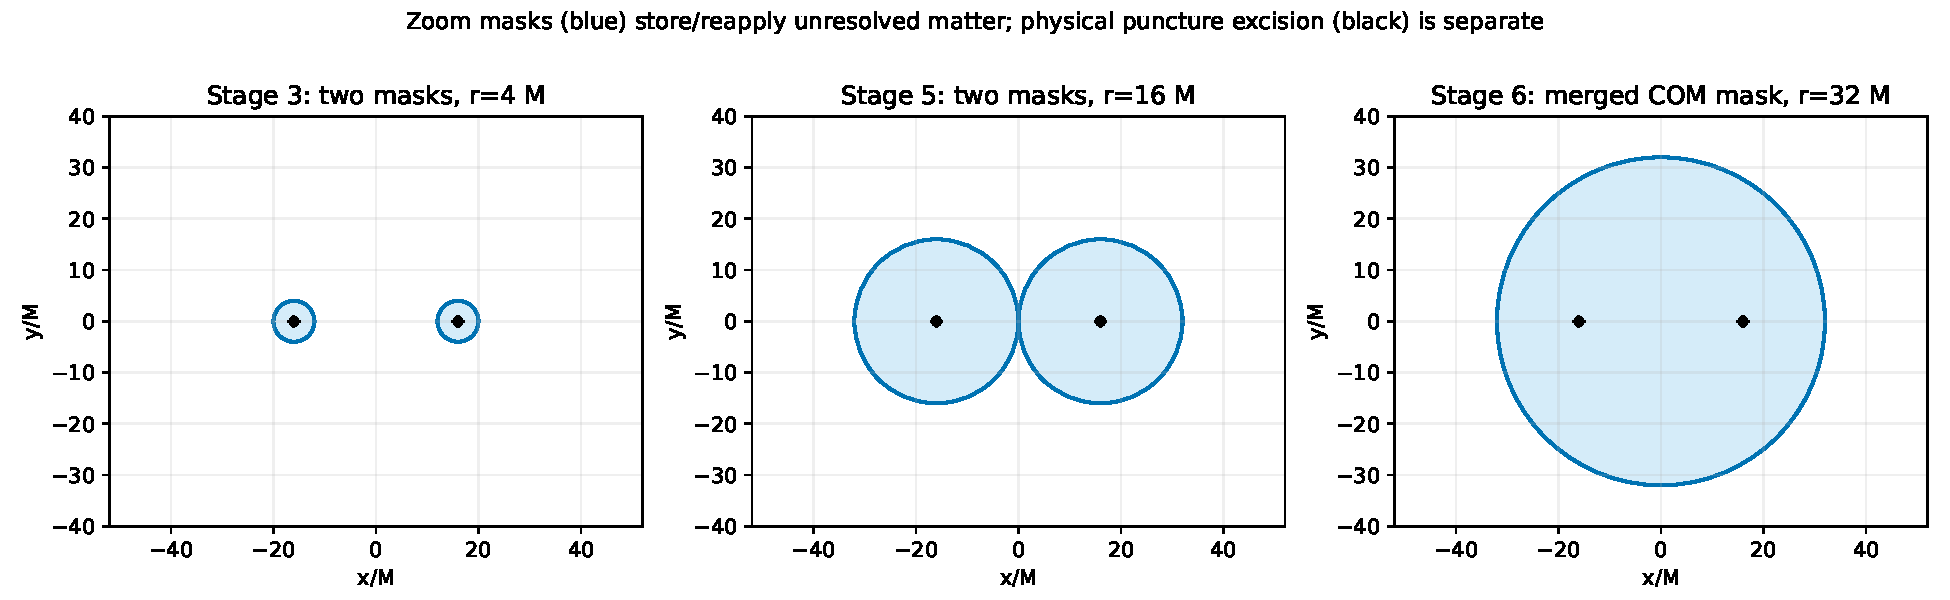
\includegraphics[width=\textwidth]{figures/mask_geometry.pdf}
\caption{Artificial masks (blue) and puncture excision (black). At $r_z<a$, separate masks follow the two coordinate-fixed holes. At $r_z\geq32M$, one COM mask encloses the previous pair. This is coordinate geometry, not a horizon finder.}\label{fig:masks}
\end{figure*}

\section{Cyclic zoom: storage, magnetic coupling, and timing}\label{sec:zoom}
The radius ladder and refinement interfaces are
\begin{equation}
 r_{z,i}=0.5\,2^iM,\quad r_{{\rm ref},i}=4r_{z,i},\quad i=0,\ldots,7.
\end{equation}
Stages $0$--$5$ use two centers; stages $6$--$7$ use the COM. A sampled angular audit found $r_z/\Delta x=16$ on all mask surfaces. This is not uniform horizon resolution: the minimum puncture cell is $m_A/16$, while cells on the nominal $r_A=1M$ sphere are $m_A/8$.

Outward zoom saves fine matter states, staggered magnetic information, and electric-field information before derefinement. During coarse evolution, cached matter primitives are reapplied inside masks and converted to conserved variables with the actual ADM geometry. Magnetic evolution still uses CT, with stored fine-to-coarse EMF information added to coarse edge fields:
\begin{equation}
 \partial_t\Btilde{\boldsymbol B}=-\nabla_h\times
 (\boldsymbol{\mathcal E}_{\rm coarse}+\delta\boldsymbol{\mathcal E}_{\rm stored}).
\end{equation}
Physical logs show \texttt{add\_emf=1}. It is therefore inaccurate to say that all masked magnetic variables are simply frozen. CT structure and unresolved EMF information are retained; exact global mass/energy conservation is not thereby proven.

Inward zoom restores stored states on the refined logical mesh, reapplies masks, and refreshes boundaries/primitives. The sequence is $0\to1\to\cdots\to7\to6\to\cdots\to0$. The finest state is not replaced by a uniform seed at every return. Native checkpoints include the active mesh and saved cyclic data. Movies show only active AMR fields, not the archived fine mesh during coarse stages.

The MHD schedule follows the structure of Equation (20) of \citet{Guo2025}, with our binary local-mass extension:
\begin{align}
 \mu_i&=\begin{cases}m_A=0.5M,&r_{z,i}<a,\\M,&r_{z,i}\geq a,\end{cases}\nonumber\\
 t_{{\rm dyn},i}&=\sqrt{r_{z,i}^3/(G\mu_i)},\nonumber\\
 \Delta t_i&=\begin{cases}
 500Gm_A/c^3=250M,&i=0,\\
 0,&i=1,2,\\
 \min(50t_{{\rm dyn},i},0.15t_B),&i\geq3.
 \end{cases}\label{eq:dwell}
\end{align}
The shared reservoir cap is $1185.854M$. Physical runs use \texttt{residence\_scale=1}; accelerated values belong only to topology tests. Zero nominal dwell still needs timestep-ordered mesh transitions.

\begin{table*}[t]
\centering\caption{Physical residence prescription on each visit}\label{tab:stages}
\begin{tabular}{rrrrrrr}\toprule
Stage & $r_z/M$ & Centers & $\mu_i/M$ & $r_{\rm ref}/M$ & $\Delta t_i/M$ & $\Delta t_i/t_{{\rm dyn},i}$\\\midrule
0&0.5&2&0.5&2&250.000&500.00\\
1&1&2&0.5&4&0&0\\
2&2&2&0.5&8&0&0\\
3&4&2&0.5&16&565.685&50.00\\
4&8&2&0.5&32&1185.854&37.06\\
5&16&2&0.5&64&1185.854&13.10\\
6&32&1&1&128&1185.854&6.55\\
7&64&1&1&256&1185.854&2.32\\\bottomrule
\end{tabular}
\end{table*}

The cap makes the largest stage only $2.32$ dynamical times, not $50$. The nominal roundtrip is $9682.35M$; the logged first finest return is $9683.038M$, including timestep overshoot. Define the finest clock
\begin{equation}
 T_{\rm fine}(t)=\int_0^t\mathbf{1}_{i(t')=0}\,dt'.\label{eq:exposure}
\end{equation}
At the retained live log, $t=10208.05M=1.29t_B=8.98P_b$, but $T_{\rm fine}=500.012M=0.440P_b$ (Figure~\ref{fig:timeline}). Each finest visit is $500$ individual-hole gravitational times. At $r_A=2M$, the illustrative Newtonian dynamical scale is $\sqrt{r_A^3/m_A}=4M$, giving $62.5$ such times per visit. This radius is inside the isolated-hole ISCO, so the estimate does not describe stable circular orbits or prove relaxation of a minidisk or magnetic flux. Half a binary orbit and many near-hole dynamical times can describe the same finest exposure.

\begin{figure*}[t]
\centering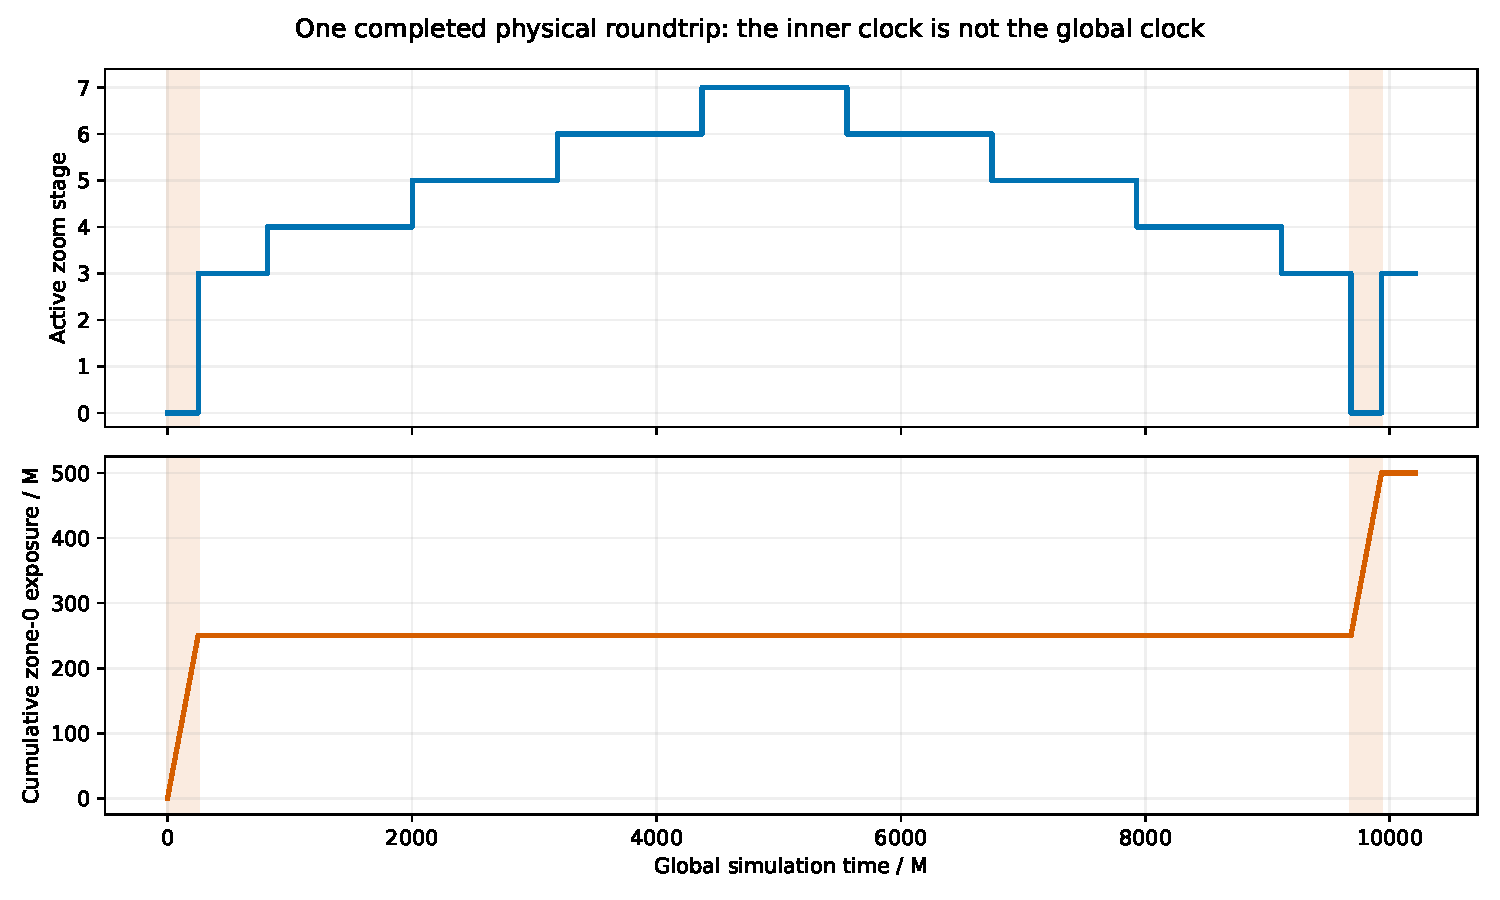
\includegraphics[width=.93\textwidth]{figures/zoom_timeline.pdf}
\caption{Logged stage history and stage-0 exposure. Shaded intervals are the two finest visits. The global clock exceeds $10^4M$ while the finest clock is only $500M$. Exposure elsewhere depends on position relative to the masks; this indicator is not a universal regional age.}\label{fig:timeline}
\end{figure*}

\section{Flow visualization and plasma beta}
Figure~\ref{fig:xy} shows the latest validated finest equatorial state. Enhanced near-hole density developed from the uniform seed. Temperature is shown as $p/(\rho c^2)$, not Kelvin without a chosen molecular weight. Valencia outputs require the conversion
\begin{align}
 B^i&=\Btilde^i/\sqrt{\gamma},\quad
 W^2=1+\gamma_{ij}\utilde^i\utilde^j,\nonumber\\
 b^2&=\frac{\gamma_{ij}B^iB^j+(\gamma_{ij}B^i\utilde^j)^2}{W^2},\qquad
 \beta_{\rm p}=2p/b^2.\label{eq:beta}
\end{align}
The movie evaluates the stationary spatial metric at each active cell center, including coarse topologies. Its nonspinning boosted-KS specialization matches saved initial components to $5.96\times10^{-8}$ normalized by $\max(1,|\gamma_{ij}|)$. Beta matches saved-ADM conversion to $1.27\times10^{-7}$ outside excision at the latest finest state. Excision interiors are not physically interpreted.

\begin{figure*}[t]
\centering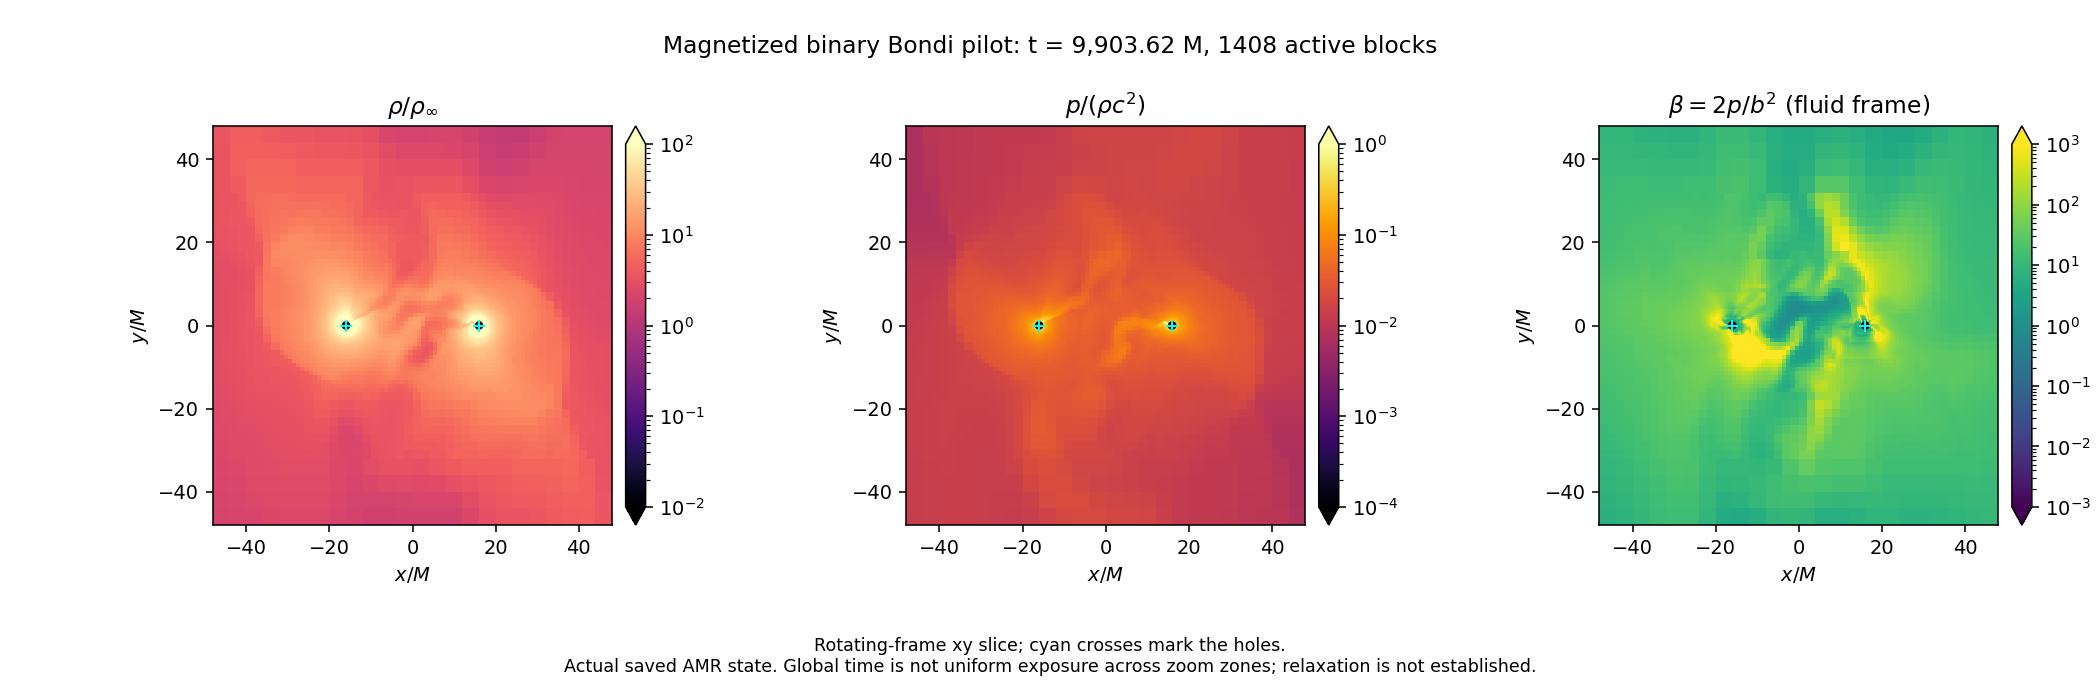
\includegraphics[width=\textwidth]{figures/flow_xy.png}
\caption{Finest $xy$ slice at $9903.62M$: density, temperature proxy, and fluid-frame beta. Crosses mark the holes and black masks denote nominal puncture excision. This is an evolving returned state, not a converged statistical average.}\label{fig:xy}
\end{figure*}

\section{Inflow-equilibrium audit}\label{sec:equilibrium}
\subsection{Measurements and matched phases}
Saved stationary ADM is reused only after exact geometry/logical-topology checks on every finest state. On rotating-coordinate spheres, positive inward rest-mass rate is
\begin{equation}
 \dot M(R)=-\int_{S_R}\rho\sqrt{\gamma}
 (\alpha\utilde^i-W\beta_s^i)n_iR^2d\Omega,\label{eq:mdot}
\end{equation}
where $n_i$ is the coordinate Euclidean normal. Near-hole spheres have $R_A=1.5,2,3M$ and centers $x_A=\pm16M$; they are not apparent horizons. COM spheres use $24,32,64,128,256,500M$. We compare $24\times48$ and $48\times96$ angular quadratures with active-cell interpolation. Angular convergence does not bound spatial interpolation error.

For fixed shells we measure
\begin{equation}
 M_{\rm sh}(R_1,R_2)=\int_{R_1<r<R_2}\rho W\sqrt{\gamma}\,d^3x.
\end{equation}
Shell edges are $24$, $32$, $64$, $128$, $256$, and $500M$; cells are assigned by their centers. Absolute shell boundaries are coarse, but meshes are identical for the temporal comparisons.

There are only two finest visits: startup ($v=0$) and first return ($v=1$). The reported comparison is the three-phase sample mean
\begin{equation}
 \overline Q_v=\frac13\sum_{s\in\{50,100,200\}M}
 \operatorname{interp}[Q_v](s),\label{eq:phase}
\end{equation}
where $s$ is time since visit entry. This is not a long-time average. Nominal output cadence is $50M$; clean-stop dumps and preserved restart counters create gaps. Linear interpolation stays within each finest visit, never across a frozen interval. Rates are raw code units; the older hydro Michel normalization is not used.

\begin{figure*}[t]
\centering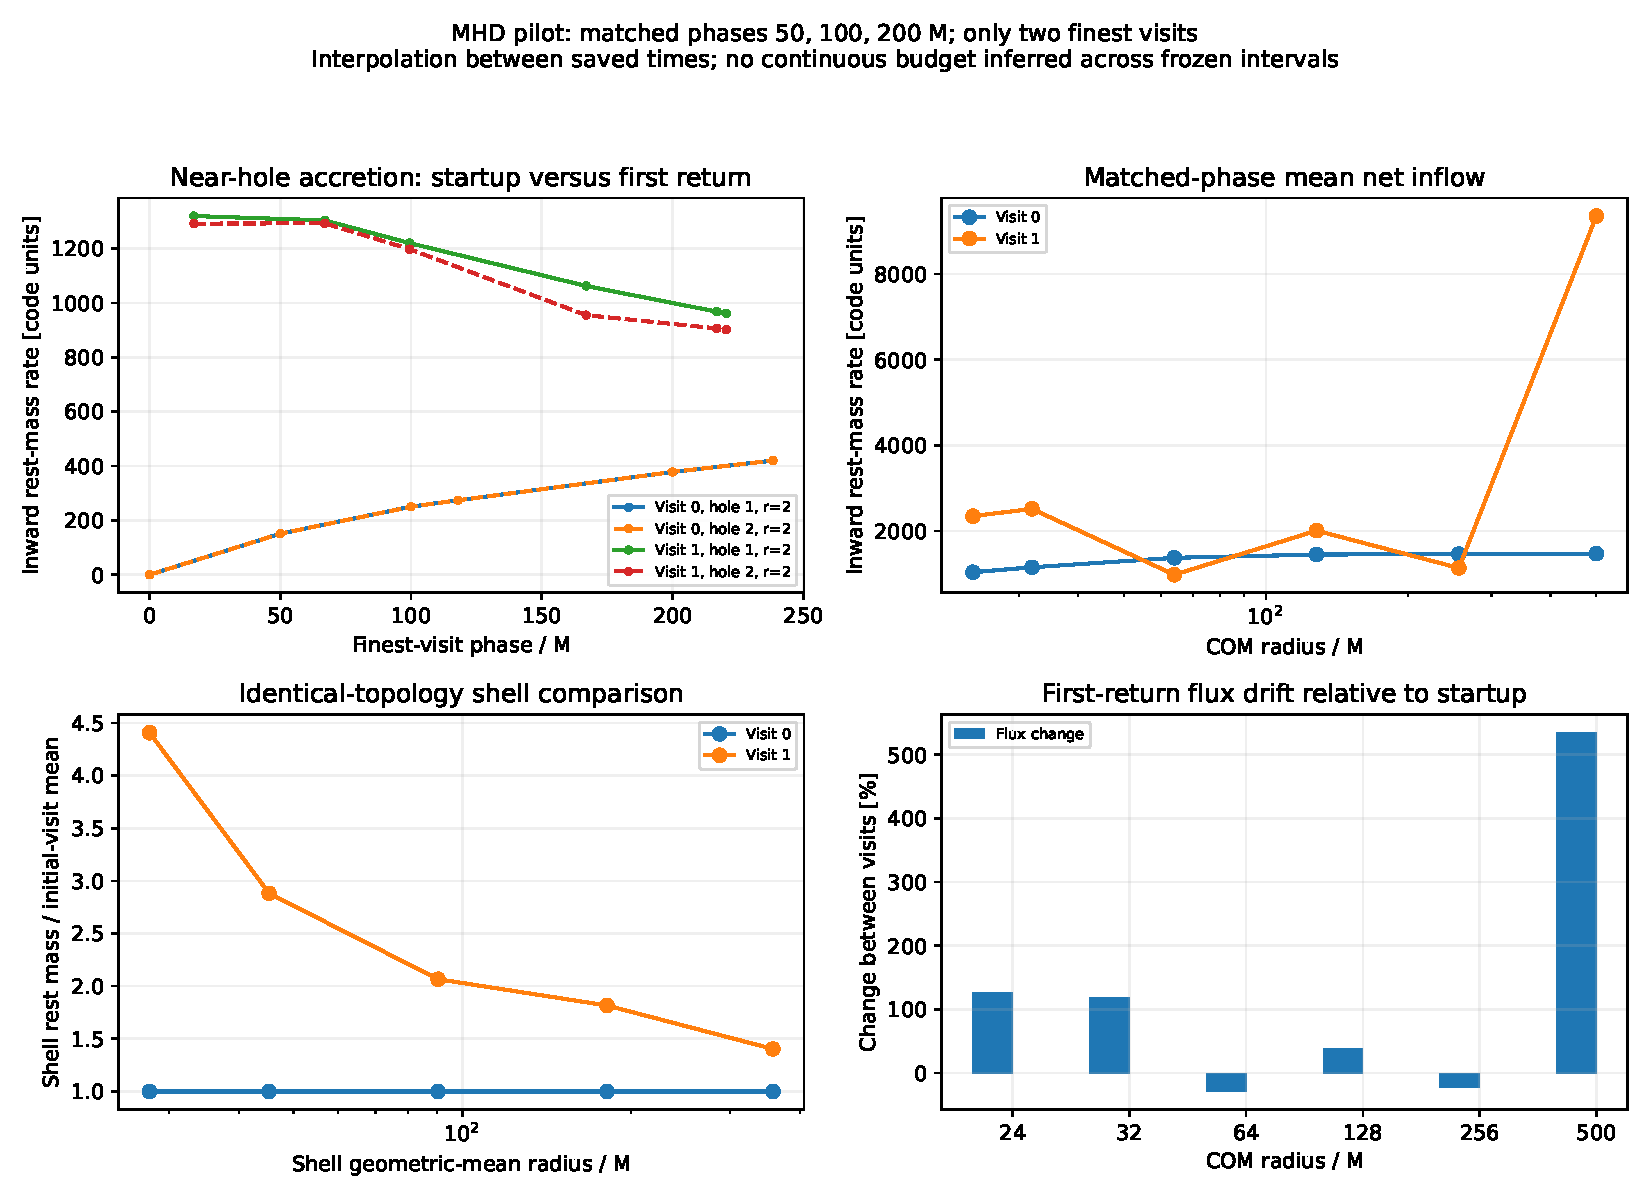
\includegraphics[width=.96\textwidth]{figures/inflow_equilibrium.pdf}
\caption{Startup versus first-return diagnostics at matched phases. Upper left: individual-hole $R_A=2M$ rates against visit phase. Upper right: COM net inflow profiles. Lower left: shell masses relative to startup-visit means. Lower right: first-return flux changes. These are different evolving states, not a continuous mass-budget residual or evidence of convergence.}\label{fig:equilibrium}
\end{figure*}

\subsection{Result: still a substantial startup transient}
At $R_A=2M$, matched-phase rates change from $(259.6,259.7)$ to $(1175.5,1136.7)$ for the two holes: factors $4.53$ and $4.38$. Returned rates decline from roughly $1300$ at phase $17M$ to $900$--$960$ at phase $221M$. Shell masses grow by factors $4.41$, $2.88$, $2.07$, $1.82$, and $1.40$, from inner to outer shell. COM rates change by about $(+126,+118,-29,+38,-22,+535)\%$ across the radii above. The outermost value compares to a starting outer flow, not two settled cycles.

First-return matched-phase mean angular sensitivities are at most $1.13\%$ in COM rates and about $0.11\%$ near the holes, far below the changes. Spatial error and asynchronous masking can contribute to radial structure, however. We cannot assign a percentage distance to equilibrium or certify an equilibrium radius. The Bondi region has experienced only about $1.3t_B$ globally. Rapid near-hole response does not establish stationary reservoir, magnetic flux, feedback, or binary-scale circulation. A fixed reservoir is not a guarantee of stationarity; magnetized accretion may instead settle statistically with persistent fluctuations.

A later audit needs several post-startup visits at matched phases, independent variability estimates, shell trends, magnetic flux, thermodynamic transport, and resolution/boundary-distance controls. For a source-free statistically stationary shell, mean \emph{net} flux is constant radially even if gross inward and outward fluxes vary. Applying this to cyclic evolution requires explicit terms:
\begin{align}
 \Delta M_{\rm sh}={}&\int(\dot M_{\rm in}-\dot M_{\rm out})dt\nonumber\\
 &+\Delta M_{\rm mask}+\Delta M_{\rm floor}+\Delta M_{\rm grid}.
\end{align}
These discrete source terms were not measured here. Differences between restored states are not a continuously measured physical accumulation rate.

\section{Outer-boundary assessment}
\begin{figure*}[t]
\centering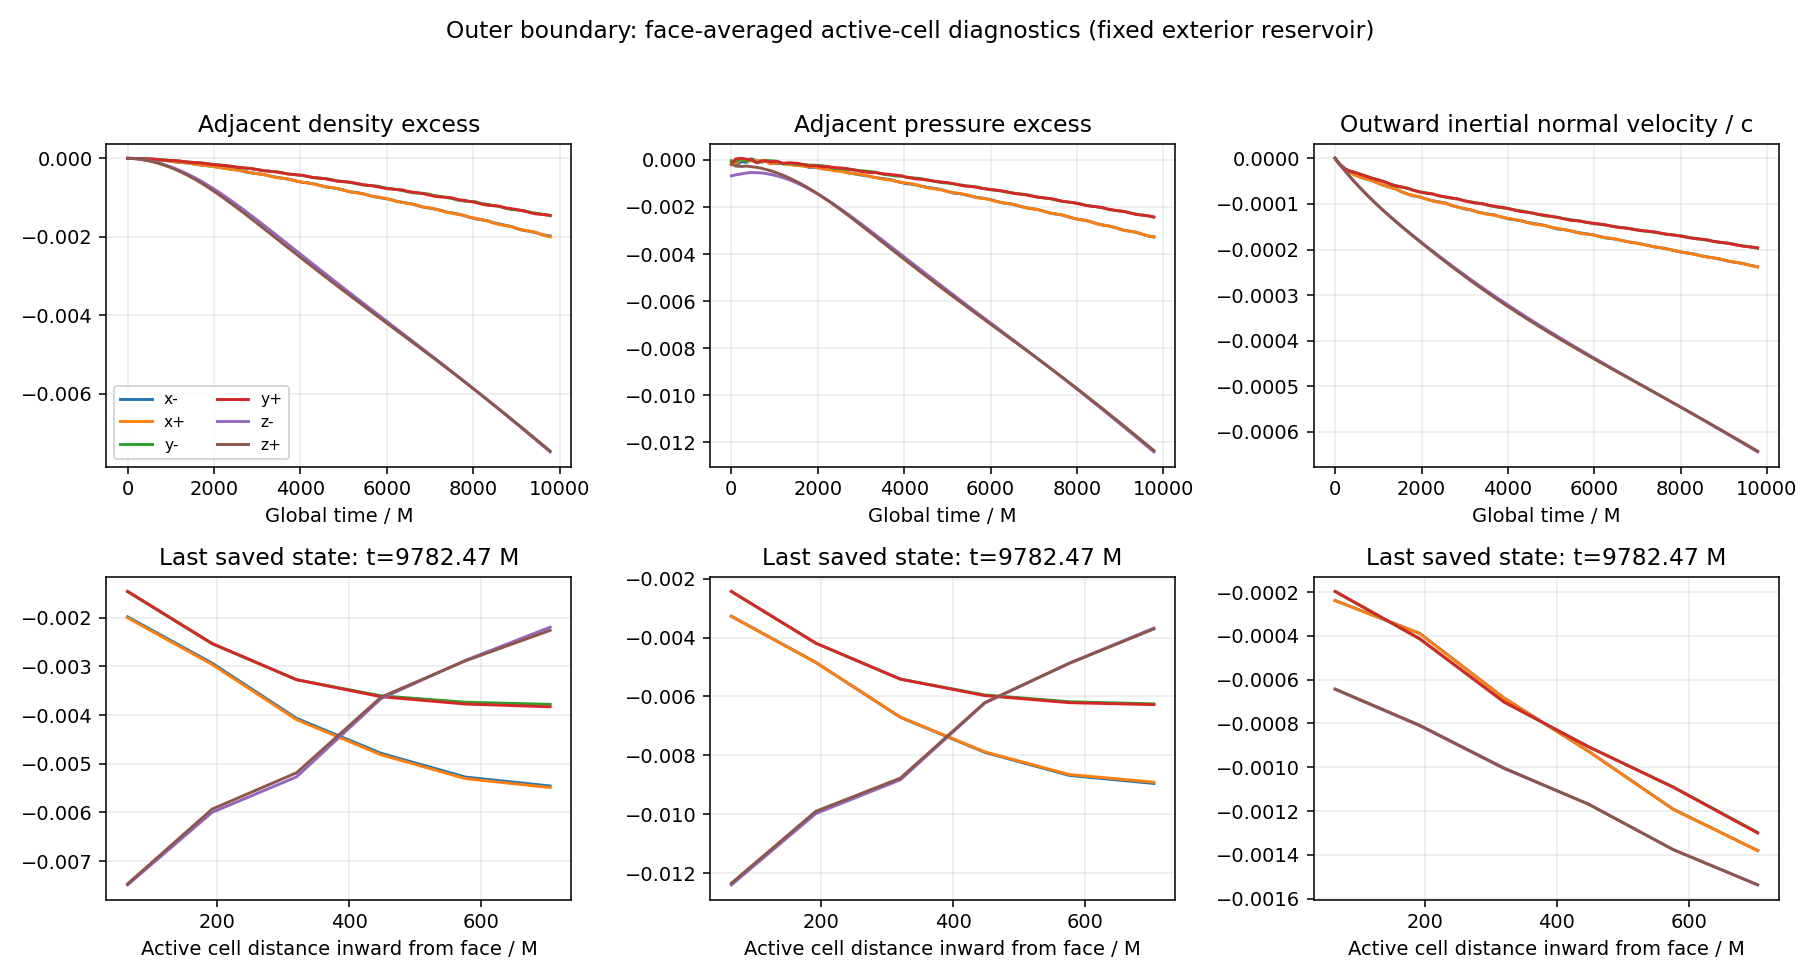
\includegraphics[width=.96\textwidth]{figures/boundary_profiles.png}
\caption{Six-face active-cell audit through $9782.47M$. Top: means versus global time; bottom: profiles inward from each face. Negative outward-normal velocity is inward motion after rotation removal. Polar depletion is smooth, but these data do not establish nonreflection or a face-flux mass budget.}\label{fig:boundary}
\end{figure*}

Faces lie at $4.096r_B$. Through $9782.47M$, adjacent cells show maximum local density/pressure departures of $1.61\%/2.66\%$, and maximum absolute face-mean departures of $0.75\%/1.24\%$. The strongest depletion is at the two faces parallel to the field. Inertial coordinate speed reaches $0.00153c$. The largest absolute face-mean departure in stored $\Btilde B_z/B_0$ is $0.234\%$, with individual-cell departure up to $1.07\%$.

Histories are smooth and opposite faces nearly agree. No large boundary instability is apparent, but a mild boundary-associated polar adjustment layer is present. One box size cannot separate its contribution from physical anisotropic inflow and seed adjustment. Initial $2\%$ noise contributes to local pressure extrema.

Figure~\ref{fig:boundary} samples active layers $64,192,\ldots,704M$ inside each face, at cell width $128M$. Ghost cells and physical face fluxes are not in these snapshots. Fixed exterior rest differs from active inflow; subsonic MHD waves can reflect. Inner contamination is not bounded. A matched-resolution larger-box comparison and characteristic/outgoing-wave control are needed before claiming boundary independence.



\section{Validation and execution record}
The accelerated full-hierarchy GPU test visited all eight stages and restored the finest topology with positive finite fluid and scaled divergence near $3.4\times10^{-15}$. It is excluded from physical-relaxation analysis. Completed physical jobs have nonzero fields, positive finite matter, twelve successful rank exits, and matched saved fluid/divergence states. The cell-centered proxy
\begin{equation}
 \epsilon_{\nabla B}=\frac{\Delta x|\nabla_h\cdot\Btilde{\boldsymbol B}|}
 {\max(|\Btilde{\boldsymbol B}|,10^{-3}B_{\rm ambient})}
\end{equation}
remains below $3.3\times10^{-12}$ through the latest completed job (gate $10^{-9}$). It is not an invariant staggered face-flux norm. Absolute puncture-field roundoff is not interpreted as physical magnetic pressure.

Each job uses only debug-scaling, one node with six physical GPUs/twelve explicit tiles, a one-hour PBS request, and Athena \texttt{-t 00:55:00}. The separate magnetic build uses the validated SANE compiler/Kokkos/MPICH environment, PPM4, HLLE, RK2, and FOFC. Accounted RSS-plus-tracked peak sums are $22.0$--$23.6$ GB; guard budgets total $28.4$ GB. This is not independent telemetry for every driver allocation.

The controller requires successful validation, matching final checkpoint, unchanged executable/core-source hashes, an empty own-user debug-scaling queue, and a unique receipt before submitting a continuation. Observation failures do not justify duplicate submissions. Other agents' jobs and the debug queue are untouched. Original source/build records, including an archived comment-only difference and an early runtime implicit-scaling omission, are retained without retroactive edits.

\section{Interpretation and next evidence needed}
Uniform inertial-rest data and external ghosts pass short frame controls. Full GPU cyclic topology and bounded physical MHD evolution work. Movies show physical beta and real active meshes. Nevertheless, there is only one full roundtrip, the finest clock is short, accretion and shell masses have changed strongly, smooth excision is off, and nominal horizon resolution is coarser than the minimum puncture cell. Equilibrium, conservative source accounting, spatial convergence, and boundary independence remain unproven. Subsequent conclusions should be based on post-startup comparisons and controlled tests, not the global clock alone.

\clearpage
\appendix
\section{Reproducibility map}
The input is \texttt{inputs/dyngr/bondi\_hierarchy/binary\_magnetized\_lowres.athinput}. Reservoir and metric logic are in \texttt{src/pgen/dynbbh.cpp}. Timing is in \texttt{src/cyclic\_zoom/zoom\_criteria.cpp}; restoration/masking and CT logic are in that directory's \texttt{zoom\_region.cpp}, \texttt{zoom\_datablock.cpp}, and \texttt{zoom\_srcterms.cpp}. Dynamic-MHD hard resets and smooth blends are in \texttt{src/eos/primitive\_solver\_hyd.hpp}, near lines 521 and 601. Defaults and weights are in \texttt{src/coordinates/coordinates.cpp} and \texttt{excision.cpp}.

Raw snapshots reside in the ignored local magnetic build-data directory. Committed job reports are in \texttt{docs/magnetic\_bondi\_validation/physical-JOB/}; movie manifests retain exact times. This package includes \texttt{schedule.json}, live-log evidence, diagnostic JSON, and figure assets. Scripts \texttt{analyze\_magnetic\_inflow.py} and \texttt{make\_magnetic\_report\_figures.py} regenerate the analysis. Older hydro-only normalization and zero-field assertions are not used.

Compile from this directory using AASTeX 7.0.1 and \texttt{latexmk -pdf magnetic\_bondi\_status.tex}. This is a multi-file manuscript with external figure assets. The formatting follows the AAS author guide, \url{https://journals.aas.org/aastexguide/}.

\begin{thebibliography}{}
\bibitem[Guo et al.(2025)]{Guo2025} Guo, M., Stone, J. M., Quataert, E., \& Springel, V. 2025, \emph{Cyclic Zoom: Multiscale GRMHD Modeling of Black Hole Accretion and Feedback}, arXiv:2504.16802v2, \url{https://arxiv.org/abs/2504.16802}
\end{thebibliography}
\end{document}
